\section{State of the Art}

CERN's mission of understanding the fundamental structure of the universe is heavily reliant on particle accelerators. The effectiveness of the experiments carried out in these accelerators is closely tied to their luminosity, as detailed in \autoref{sec:luminosity}. This section aims to provide an overview of the luminosity measurement methods and explain how these measurements are conducted specifically in the CMS experiment.

\subsection{The van der Meer Scan Method and the van der Meer Framework}
\label{subsec:vdM}

In practice, the visible cross section is calculated using the van der Meer (vdM) scan method. This method, originally proposed by Simon van der Meer, introduces a novel way to measure the $\Sigma_X$ and $\Sigma_Y$ of the bunch overlap \cite{vanderMeer:296752}, expanding the work in \cite{Rubbia:1025746}, and thus $A_{eff}$. It works under the assumption that the transverse proton bunch density distributions are factorizable into x and y separate distributions. This method is not only used by the CMS experiment but also by all the other LHC experiments \cite{Maettig:1513982,TheLHCbcollaboration_2014,ALICE-PUBLIC-2021-001}.

\subsubsection{Van der Meer Scan Method}
\label{subsubsec:vdm-method}

A vdM scan consists of incremental shifts of the beams with respect to each other in the transverse plane. The collisions are then recorded and the rates, $R$, are measured by the luminometers. An example of a vdM scan is shown in figure \ref{fig:vdm-scan-steps}.

\begin{figure}[h]
    \centering
    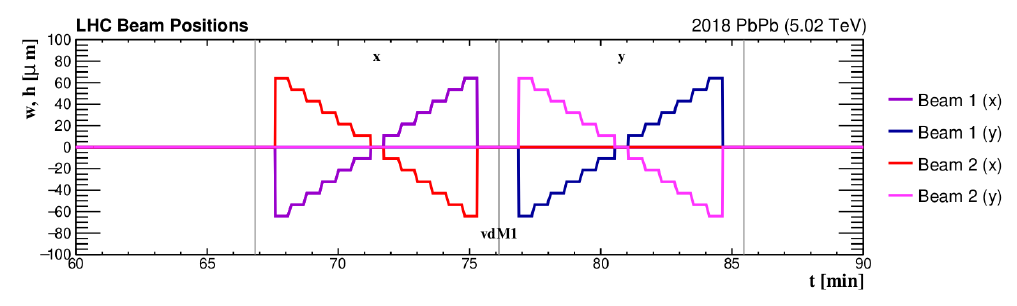
\includegraphics[width=0.8\textwidth]{sections/images/vdm_scan_steps.png}
    \caption{LHC beam positions during a vdM scan (from \textit{Ref.} \cite{Saariokari:2826125}).}
    \label{fig:vdm-scan-steps}
\end{figure}

When the beam positions in the scan plane are the same, they are said to be in the head-on position. This corresponds to the maximum overlap between the beams and thus the maximum recorded rates. The visible cross section for a given luminometer can then be calculated as:
\begin{equation}
    \label{eq:vis-cross-section-vdm}
    \sigma_{vis} = \frac{2 \pi \Sigma_X \Sigma_Y R_{\mathrm{peak}}}{N_1 N_2 f_{rev}}
\end{equation}
Here, $\Sigma_X$, $\Sigma_Y$ and $R_{\mathrm{peak}}$ are obtained by fitting a Gaussian distribution to the measured rates as a function of beam-beam separation and extracting the fit parameters. $R_{\mathrm{peak}}$ corresponds to the average peak rate at the head-on position from both directions in the transverse plane. If we consider the beams to be round, we have $\Sigma_X = \Sigma_Y = \sqrt{\epsilon_N \beta^*/ \gamma}$. $\gamma$ is the relativistic Lorentz factor, and $\beta^*$ corresponds to the value of the optical function $\beta$ at the IP. $\epsilon_N$ is the normalized transverse emittance, valued at $3.75 \mu m$ for the LHC \cite{Brüning:782076}. The visible cross-section is then used to convert the measured rates to luminosity using equation \ref{eq:luminosity-from-rates}.

\subsubsection{Corrections to Luminosity}
\label{subsub:corrections}

The vdM scans are subject to a multitude of systematic effects that ultimately affect the luminosity measurements. In order to mitigate these effects, a series of corrections are applied to both the measured rates and the beam current. For any correction that is applied, the error is propagated to the luminosity measurement. What follows is a brief description of some of the applied corrections. A detailed explanation of all these corrections can be found in \cite{Sirunyan:2759951,Saariokari:2826125}.

% \paragraph{Beam Current Calibration and Spurious Charges}

% The beam current is measured from two different devices. The Fast Beam Current Transformer (FBCT) \cite{Gras:1379466} can measure the beam current bunch-by-bunch while the Direct-Current Current Transformer (DCCT) \cite{Odier:1183400} measures the overall sum of the beam current. Since DCCT is more accurate, the FBCT measurements are calibrated to match the DCCT measurements.

% The 3564 bunches in a beam, spaced by $25ns$, are composed of 10 $2.5ns$ RF buckets. If a bunch is to be filled, typically only the first bucket contains all the particles. However, spurious particles can be present in the other buckets. These are called satellite charges while particles in nominally empty buckets are called ghost charges. These particles cause an overestimation of the beam current which is corrected by applying a correction factor to the measured current.

\paragraph{Background Correction}

Background signal, be it beam-induced, detector noise or machine-induced, is typically present in the raw recorded rates. This background is posteriorly subtracted from the measured rates. This signal can be measured by inspecting non-colliding bunches in the beam or even by using super separation scans where the beams are maximally separated in the transverse plane.

\paragraph{Beam-Beam Effects}

The two effects that are considered here are the beam-beam deflection and the evolution of $\beta^*$ normally referred to as \textit{dynamic}-$\beta$ effect. The former is caused by an angled kick that is induced by the electromagnetic repulsion between the two beams, changing the beam-beam nominal separation. The latter is caused by a change in the particle density distribution of the bunches at the IP which affects the value of $\beta^*$ resulting in a change in the effective transverse area. The corrections to these effects increased the measured value of $\sigma_{\mathrm{vis}}$.

\paragraph{XY-Factorization Bias}

The vdM scan method calculates the effective transverse area, $A_{eff}$, with the assumption that the bunch proton density distributions are factorizable in the transverse plane as described in \autoref{subsec:vdM}. If this assumption is not true, the calculated value for $A_{eff}$ will be biased. This bias is corrected by measuring $A_{eff}$ with two separate methods, the Beam-Imaging method \cite{Klute_2017} and the Luminous Region method discussed in \cite{Aaboud2016}. The results from these methods are used to arrive at a correction factor that is applied to the calculated value for $A_{eff}$.

\subsubsection{Van der Meer Framework}

The BRIL (Beam Radiation Instrumentation and Luminosity) group within CMS developed a specialized software tool, the VdMFramework, aimed exclusively at conducting analyses and computations for luminosity measurements. This software is an integral part of the CMS collaboration.

Started in 2015 as a self-sufficient tool, the VdMFramework was tailored to analyze vdM scans. Since its introduction, it has been continuously updated with new features, while ensuring compatibility with data from earlier data collection periods. Up to the present day, the software has undergone consistent enhancements. As detailed in \autoref{sec:activities}, a significant portion of my work at CERN is dedicated to its ongoing development and maintenance.

The VdMFramework is developed in Python 3 \cite{Python3}, incorporating ROOT, a powerful data analysis application from CERN. Its primary function includes calculating the visible cross-section, $\sigma_{\mathrm{vis}}$, and implementing various corrections as outlined in \autoref{subsub:corrections}. The software is designed to process data in Hierarchical Data Format (HDF5) \cite{koranne2011hierarchical}. This format includes critical components such as luminometer readings, beam or bunch currents, and specific details pertinent to each vdM scan, like beam-beam separation and the step intervals of the scan.

The flow of the framework begins with the reading of the data file. Following this, it generates intermediate files based on the input provided. These files cover an array of information, including conditions of the scan, beam currents, luminometer rates, and data related to necessary corrections. The software then applies the requested adjustments to the luminometer rates and produces ROOT graph files that represent these corrected rates.

Subsequently, it undertakes the fitting of a function to the rate data, as detailed in \autoref{subsubsec:vdm-method}. While Gaussian functions are commonly used, the software is also equipped to handle a variety of other fitting functions. The final step in the process involves the calculation of $\sigma_{\mathrm{vis}}$, using the peak rate and beam widths determined from the fit results. All the results are stored in files for inspection and further analysis.

An example of a fit produced by the framework, illustrating its capabilities, is presented in \autoref{fig:vdm-example-fit}.

\begin{figure}[h]
    \centering
    \begin{subfigure}[b]{0.45\textwidth}
        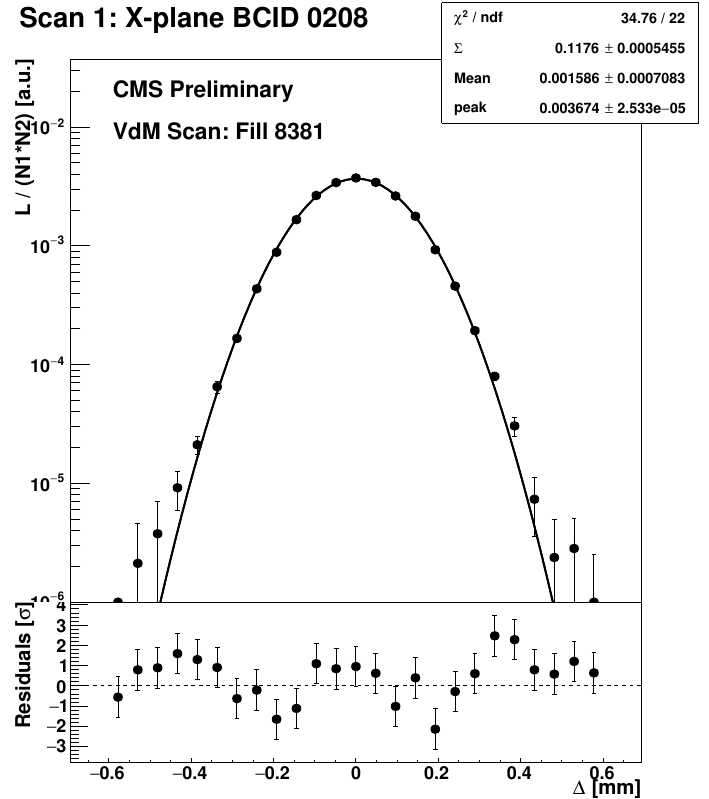
\includegraphics[width=\textwidth]{sections/images/fit_sg.png}
        \caption{}
        \label{fig:vdm-example-fit-sg}
    \end{subfigure}
    \hfill
    \begin{subfigure}[b]{0.45\textwidth}
        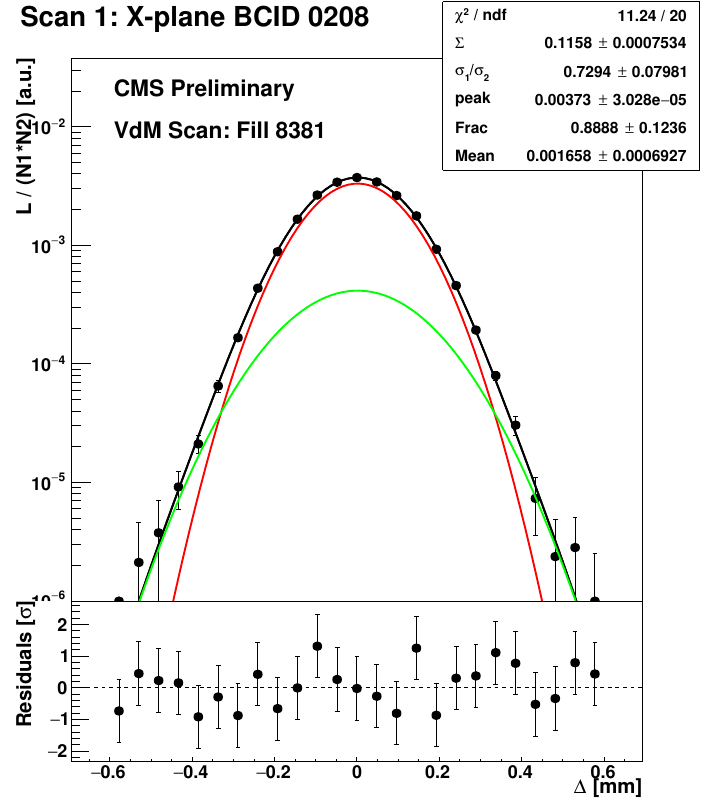
\includegraphics[width=\textwidth]{sections/images/fit_dg.png}
        \caption{}
        \label{fig:vdm-example-fit-dg}
    \end{subfigure}
    \caption{Example fit produced by the VdMFramework. The y-axis contains the normalized rates for the PLT luminometer and the x-axis the beam-beam separation. \autoref{fig:vdm-example-fit-sg} shows the fit using a single Gaussian function while \autoref{fig:vdm-example-fit-dg} shows the fit using a double Gaussian function. }
    \label{fig:vdm-example-fit}
\end{figure}

\subsection{Zero Counting Method}
\label{subsec:zero-counting}

Due to the constraints in the read-out electronics of the luminometers, there's a chance that simultaneous particle hits might be recorded as a single event. This necessitates a more advanced approach to counting hits accurately. It is postulated that the distribution of the number of hits can be modeled by a Poisson distribution \cite{TheLHCbcollaboration_2014} with mean, $\mu$, that is proportional to luminosity.
\begin{equation}
    \label{eq:luminosity-from-hits}
    \mathcal{L}_b = \frac{\mu f_{rev}}{\sigma}
\end{equation}
The zero-counting method is based on this assumption. It consists of calculating the probability that a luminometer records zero hits, $P_0$, regardless of the number of collisions that occur. This probability is given by the following equation:
\begin{equation}
    \label{eq:zero-counting}
    P_0 = \sum_{i=0}^{\infty} \frac{\mu^i e^{-\mu}}{i!} p^i = e^{-\mu(1-p)}
\end{equation}
$\mu$ is the mean number of hits per bunch crossing and $p$ is the probability that no observables are recorded in a bunch crossing with $i$ interactions. It then follows that luminosity is proportional to the natural logarithm of $P_0$:
\begin{equation}
    \label{eq:luminosity-from-hits-2}
    \mathcal{L}_b = \frac{\mu f_{rev}}{\sigma} = - \frac{\log (P_0)}{1-p} \frac{f_{rev}}{\sigma} = - \log (P_0) \frac{f_{rev}}{\sigma_{\mathrm{vis}}}
\end{equation}
The value of $p$ is here absorbed into the visible cross section \cite{Sirunyan:2759951} and does not need to be known beforehand. As we will see in \autoref{subsec:cms_detectors}, this method is frequently used in the CMS experiment to obtain the rates of the luminometers.

\subsection{Detectors at the CMS Experiment}
\label{subsec:cms_detectors}

The BRIL group at CMS, is responsible, among other things, for providing the luminosity measurements. As mentioned in \autoref{subsec:calibration}, these measurements are largely dependent on the use of luminometers to record the byproducts of the collisions.

One of the dedicated luminosity detectors is the Pixel Luminosity Telescope (PLT) \cite{CMS-DP-2021-020}. This monitor is based on the use of silicon pixel sensors, 48 in total, arranged in groups of 3 in a telescope-like structure. The sensors are placed at a distance of $1.75m$ from both ends of the IP and placed parallel to the beam axis such that any particles produced in the collisions will pass through all 3 sensors.

The Fast Beam Conditions Monitor (BCM1F) \cite{CMS-DP-2022-033} can measure not only the luminosity but also the beam-induced background. It consists of 24 silicon sensors arranged in 2 rings around the beam pipe at a distance of $1.8m$ from the IP. At this distance, the hits from the collisions can be separated from the beam-induced background. The measurements are read from two different back-end systems, the Versa Module Europa (VME)  and $\mu$TCA.

Another luminosity detector is the Hadron Forward (HF) calorimeter. This detector is composed of two steel/quartz-fiber calorimeters, one on each side of the IP, at a distance of $11.2m$ from the IP covering the pseudorapidity range $3.0 < |\eta| < 5.2$. Also using separate read-out systems, the HF calorimeter can provide luminosity measurements based on two different methods: The occupancy method (HFOC) \cite{Sirunyan:2759951} counts the fraction of channel measurements that are above a certain threshold. The transverse energy method (HFET) used the sum of the transverse energy measured in the calorimeter.

The raw data recorded by PLT, BCM1F and HFOC are converted to luminosity via the zero counting method described in \autoref{subsec:zero-counting}.

Other subsystems in the CMS detector include the CMS tracker, responsible for tracking the trajectories of charged particles, the muon system, in charge of estimating the number of muons produced in the collisions and the Radiation Monitoring System for the Environment and Safety (RAMSES), which monitors the radiation levels in the CMS cavern. Detailed descriptions of these systems can be found in \cite{TheCMSCollaboration_2008}.
